\chapter{Результаты исследования}

На рисунке \ref{img:1} представлено распределение степеней узлов исходного графа.

\begin{figure}
	\begin{center}
		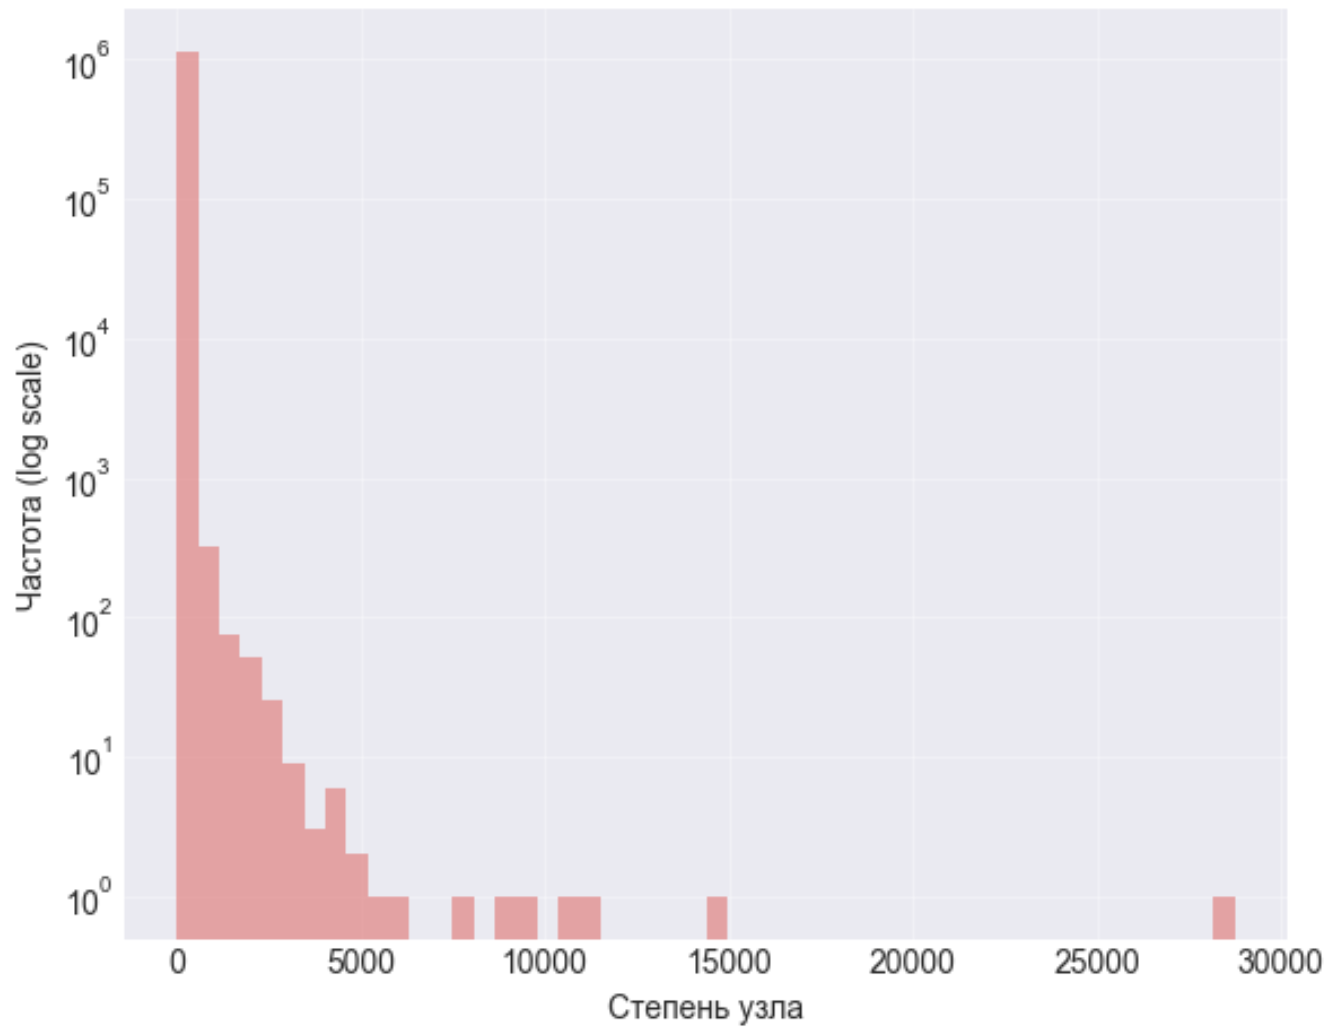
\includegraphics[width=\textwidth]{images/1.png}
	\end{center}
	\caption{Распределение степеней узлов исходного графа}
	\label{img:1}
\end{figure}

На рисунке \ref{img:2} представлена визуализация случайного подмножества из 10000 тысяч узлов графа (только 352 из них оказались неизолированными).

\begin{figure}
	\begin{center}
		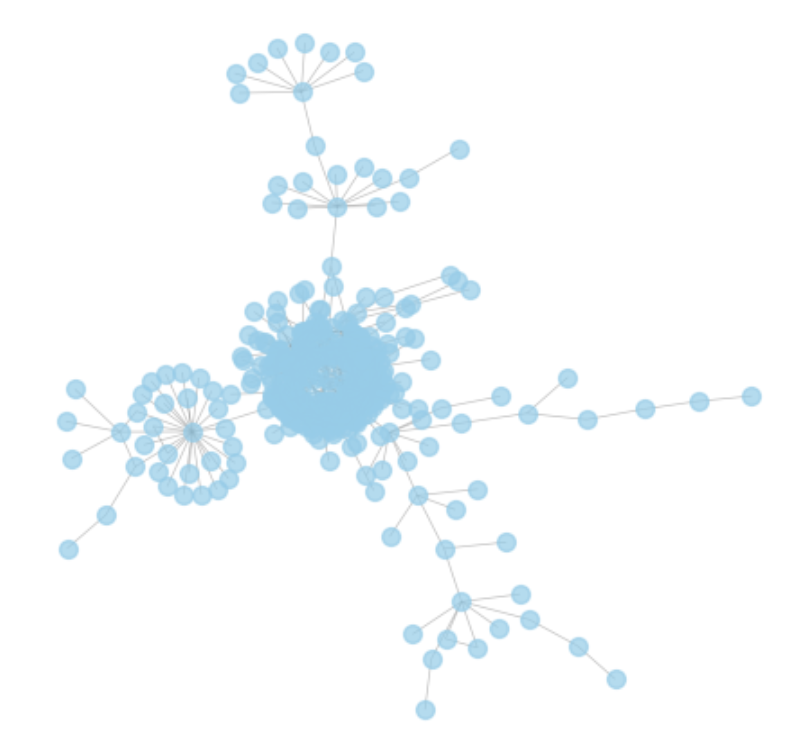
\includegraphics[width=\textwidth]{images/2.png}
	\end{center}
	\caption{Визуализация случайного подмножества графа (352 неизолированных узла)}
	\label{img:2}
\end{figure}

На рисунках \ref{img:2}-\ref{img:3} представлено распределение размеров найденных сообществ.

\begin{figure}
	\begin{center}
		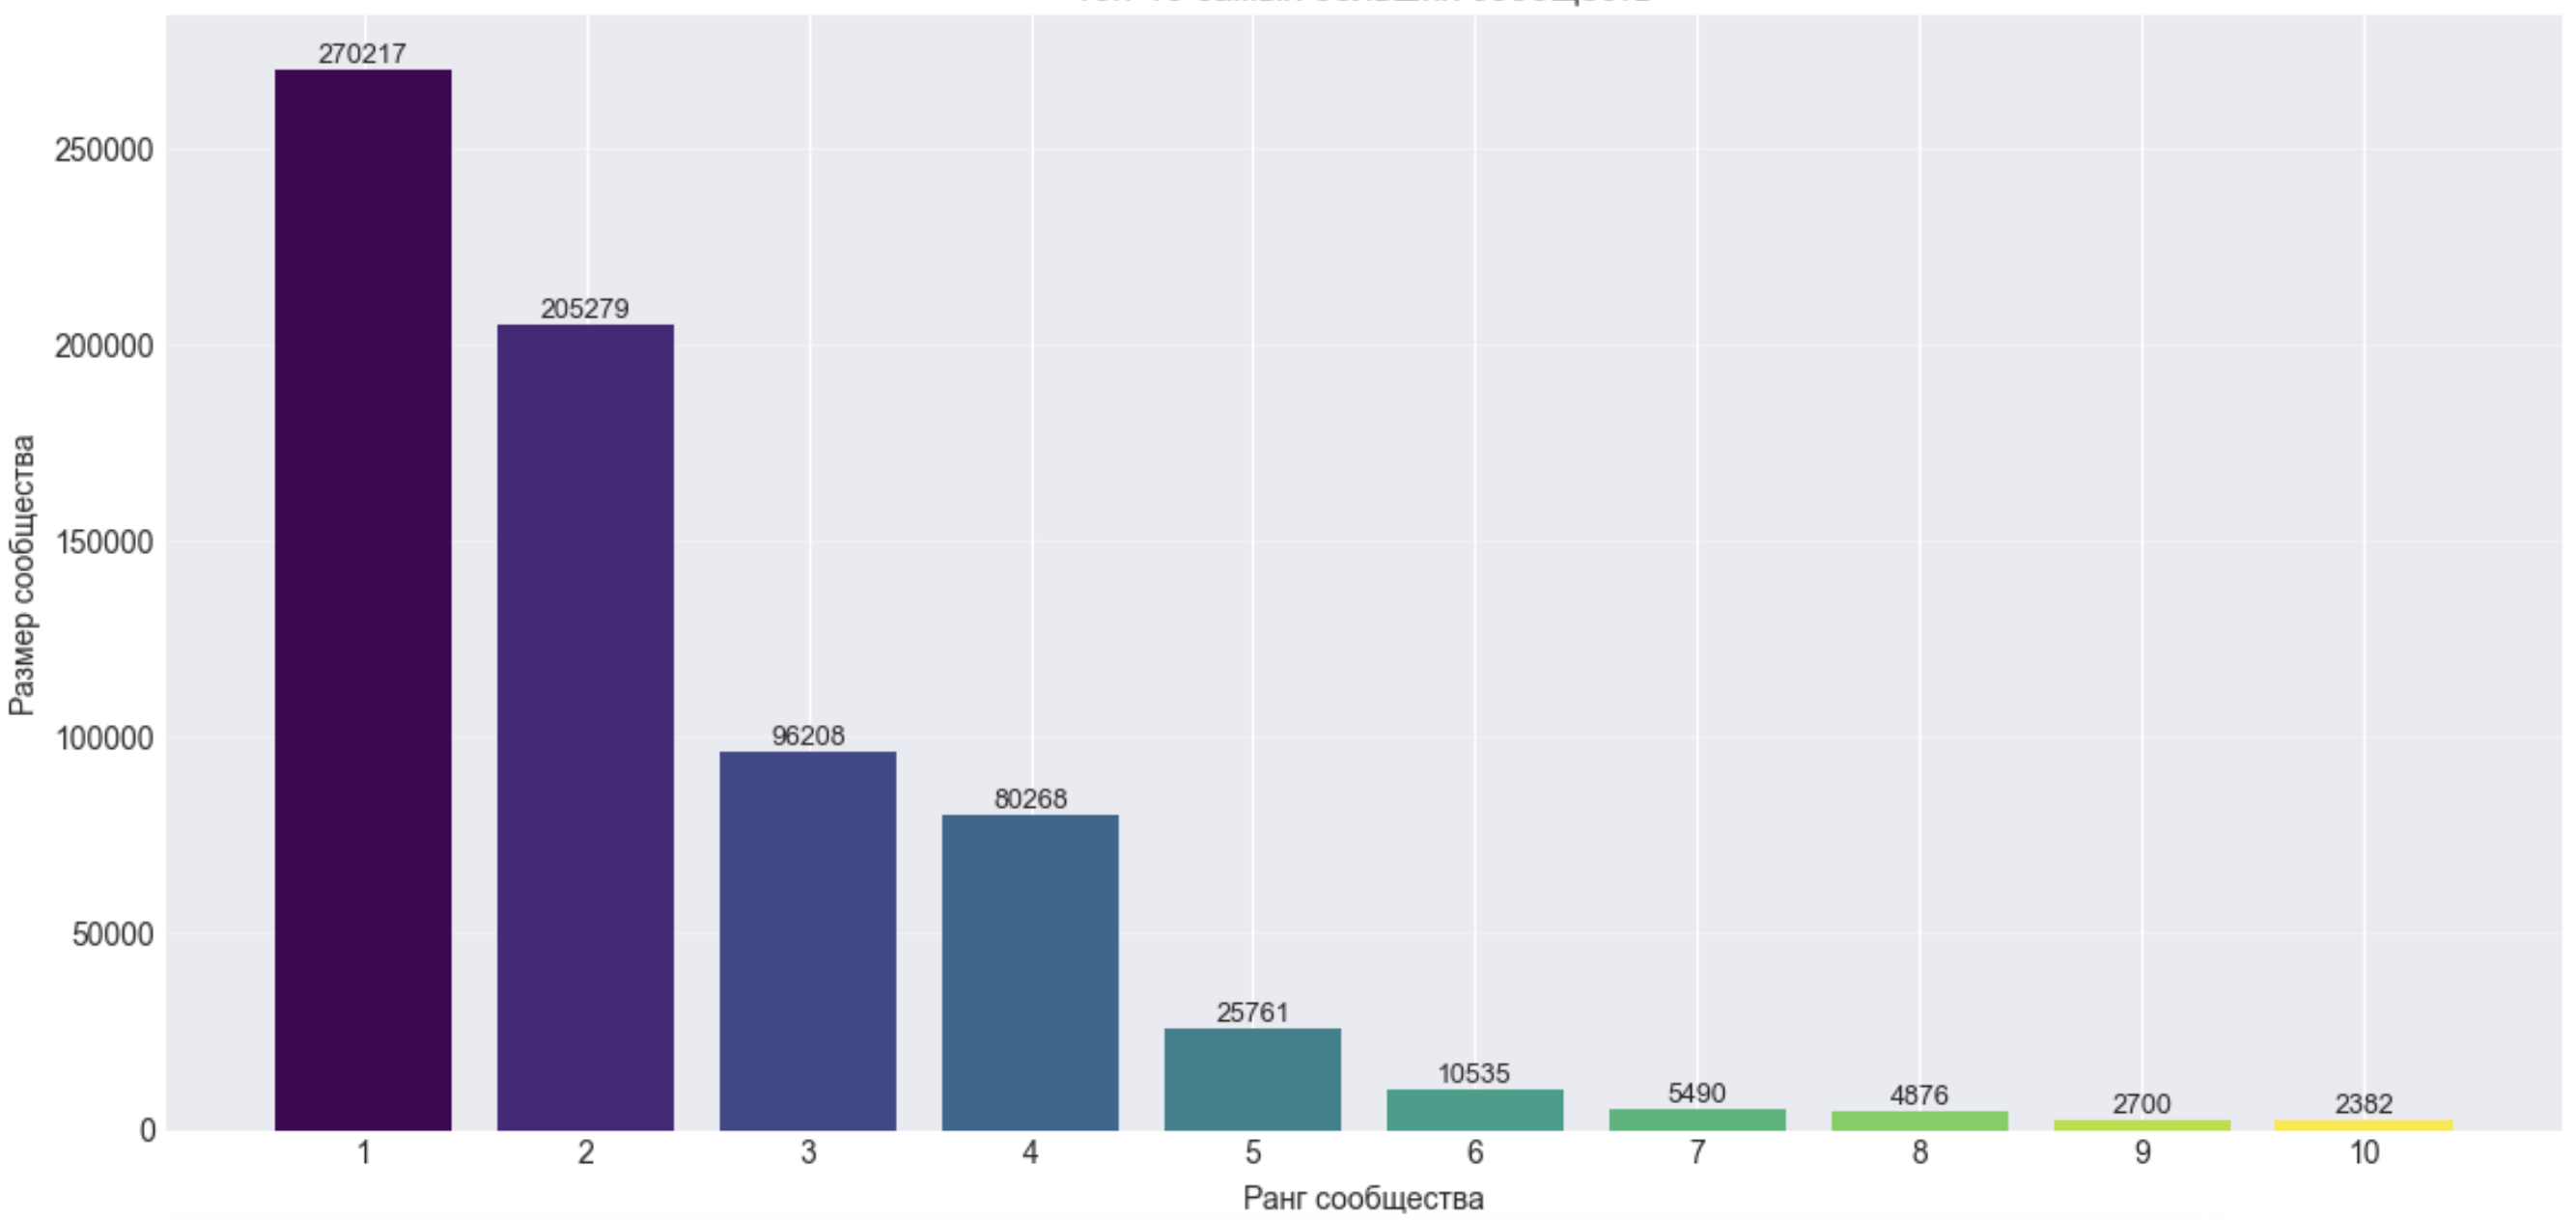
\includegraphics[width=\textwidth]{images/3.png}
	\end{center}
	\caption{Размеры 10 самых больших выделенных сообществ}
	\label{img:3}
\end{figure}

\begin{figure}
	\begin{center}
		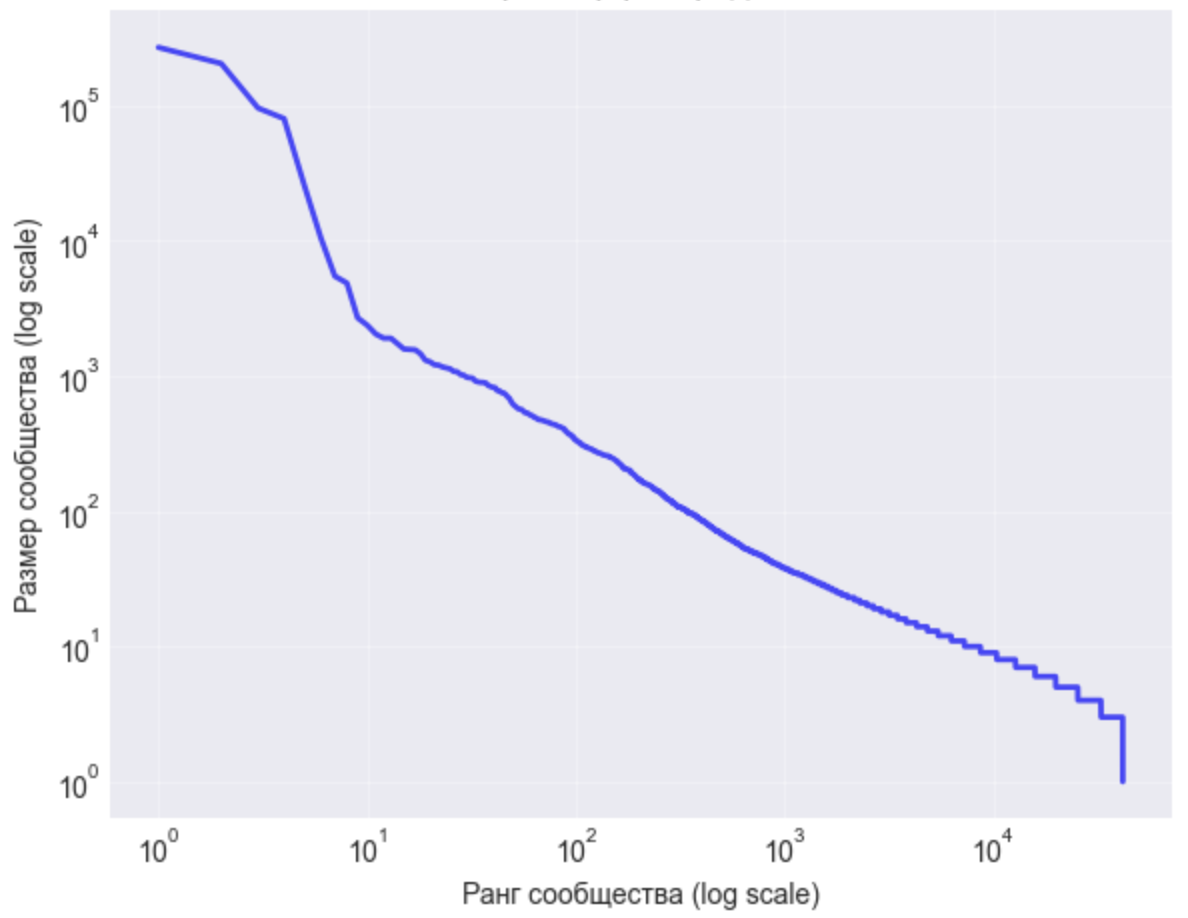
\includegraphics[width=\textwidth]{images/8.png}
	\end{center}
	\caption{Распределение размеров сообществ}
	\label{img:4}
\end{figure}

На рисунках \ref{img:5}-\ref{img:7} представлена визуализация 10, 9 и 8 по величине сообществ.

\begin{figure}
	\begin{center}
		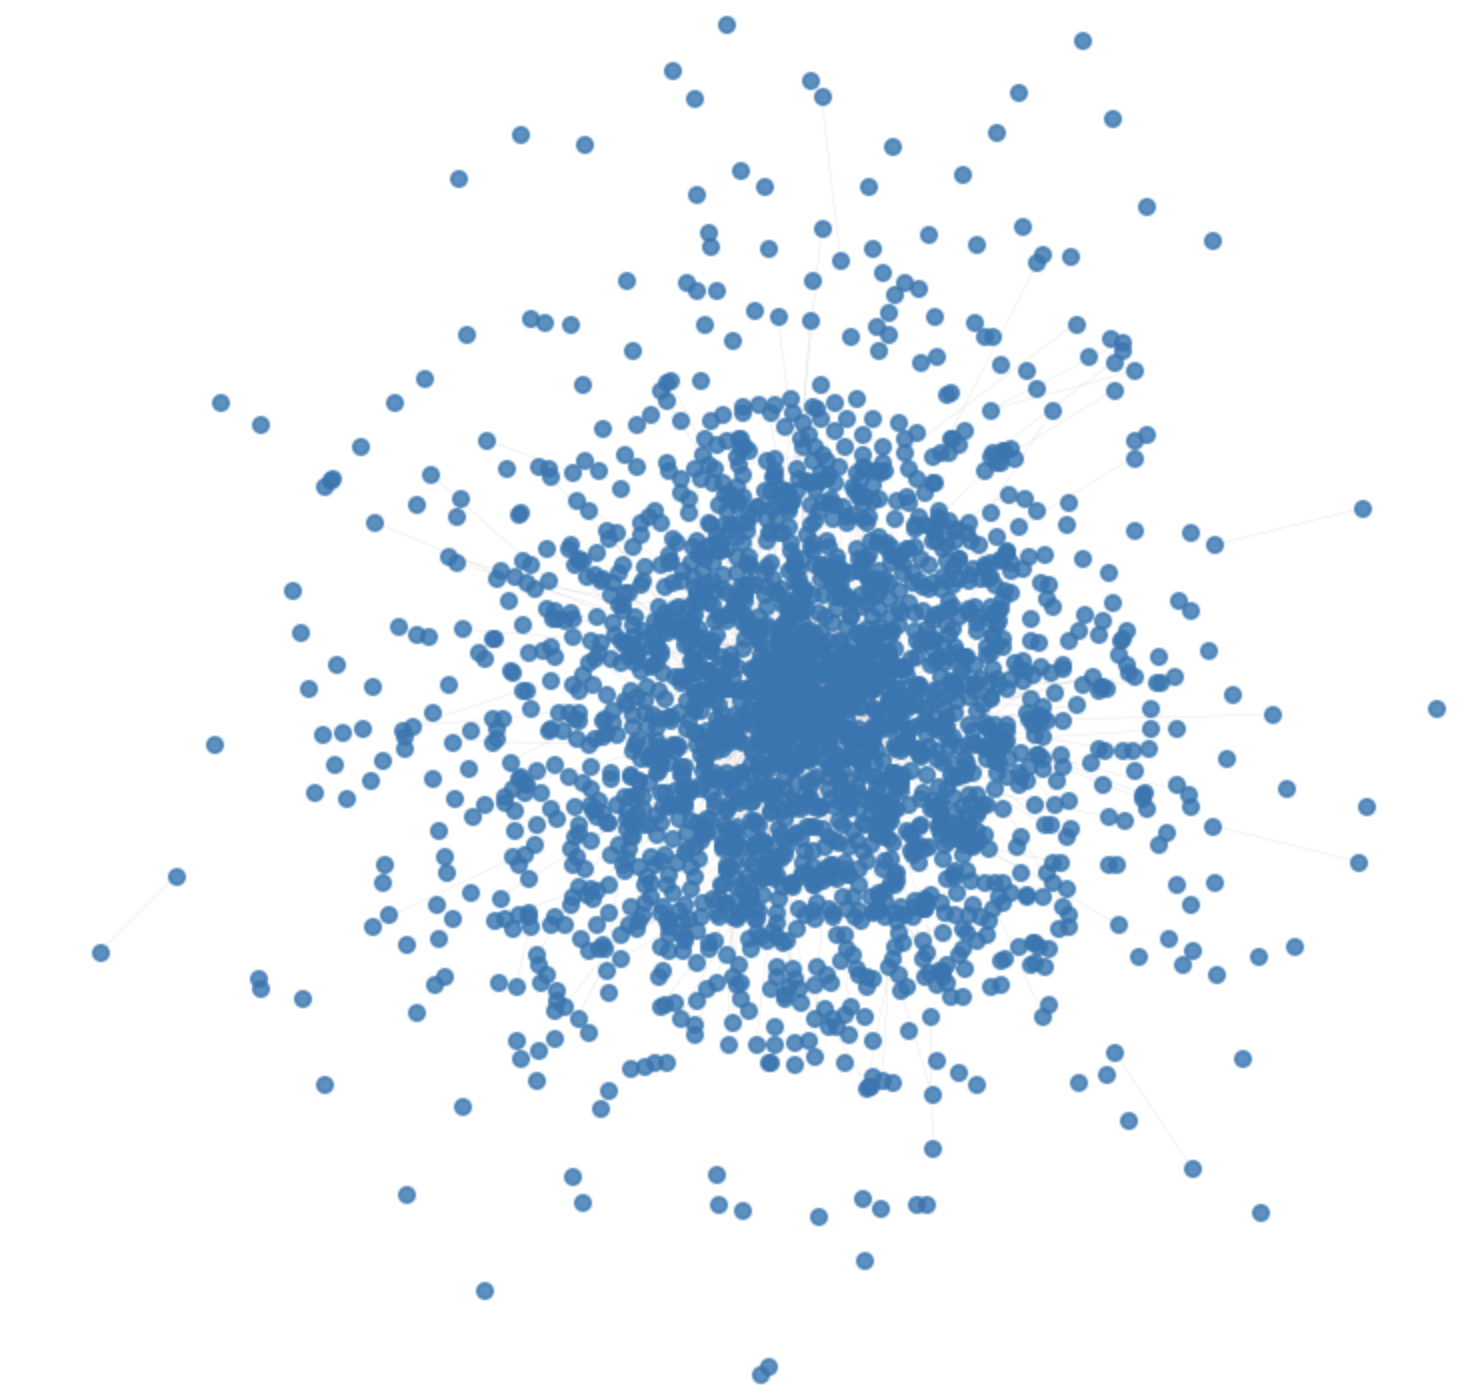
\includegraphics[width=\textwidth]{images/5.png}
	\end{center}
	\caption{Визуализация десятого по величине сообщества (2 382 узла)}
	\label{img:5}
\end{figure}

\begin{figure}
	\begin{center}
		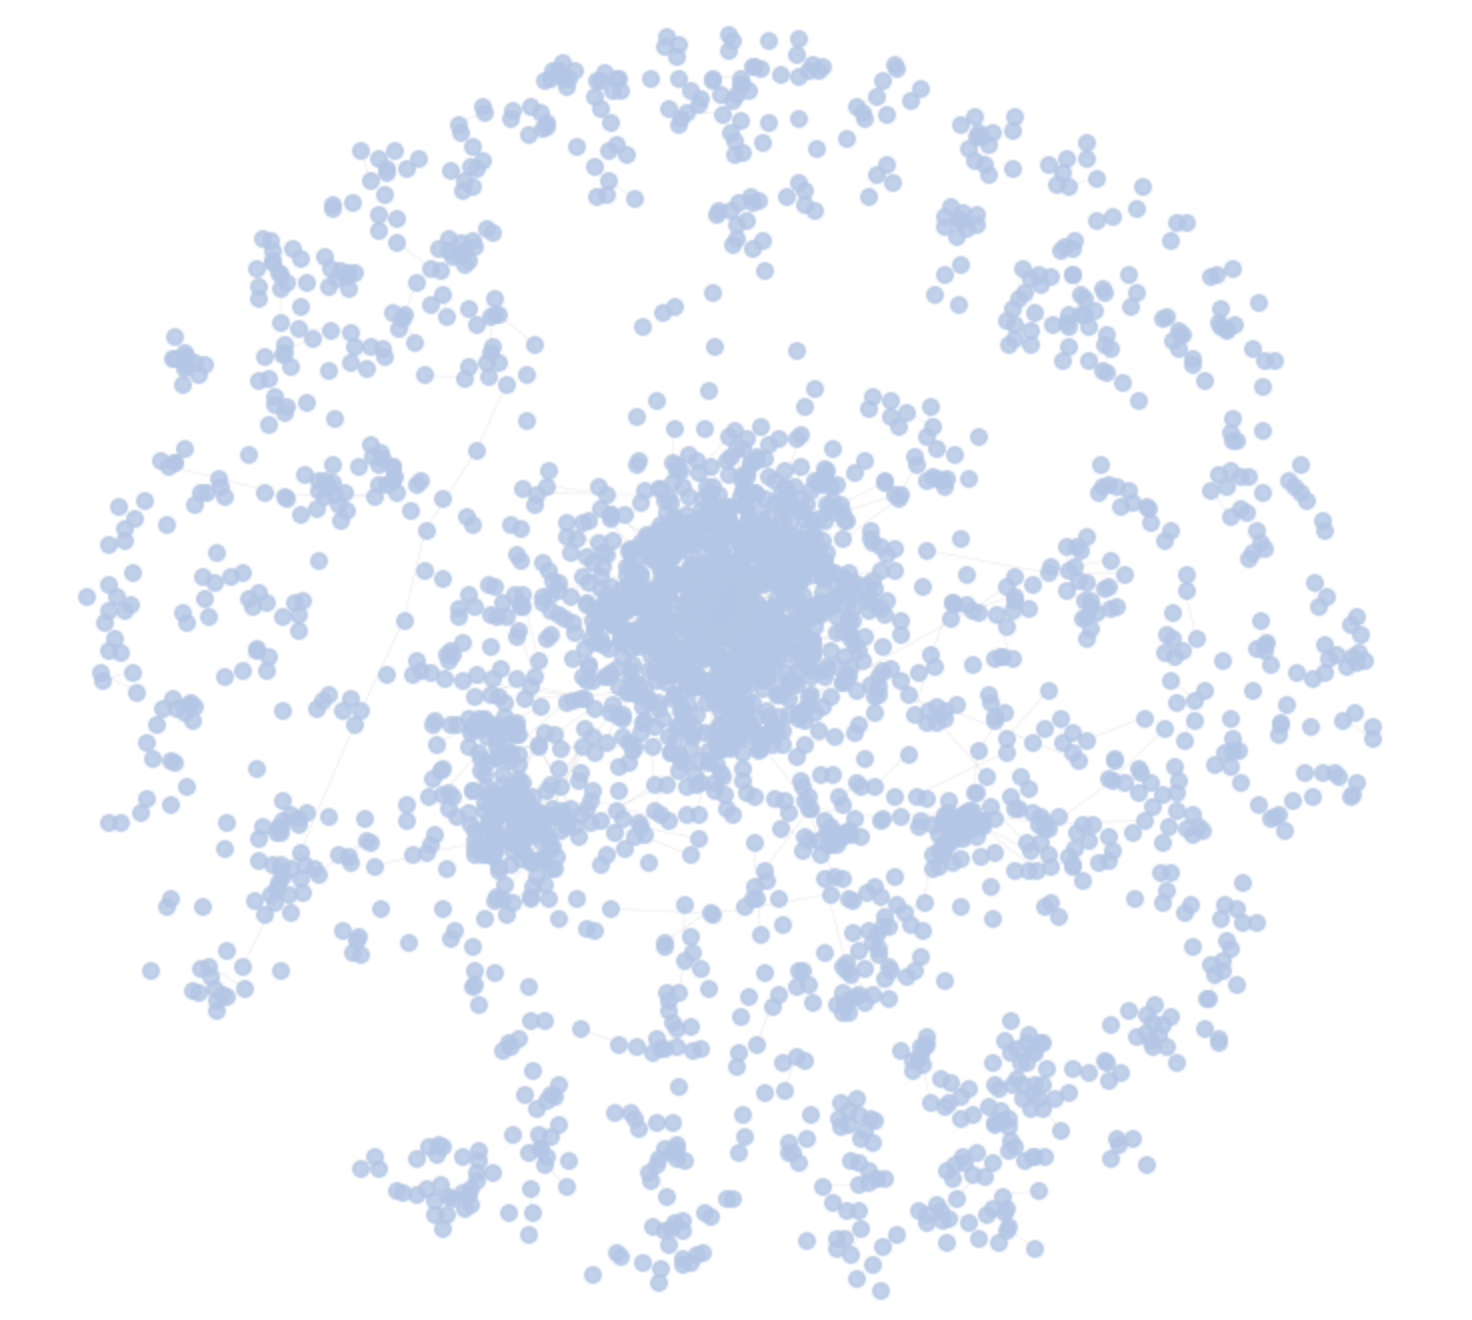
\includegraphics[width=\textwidth]{images/6.png}
	\end{center}
	\caption{Визуализация девятого по величине сообщества (2 700 узлов)}
	\label{img:6}
\end{figure}

\begin{figure}
	\begin{center}
		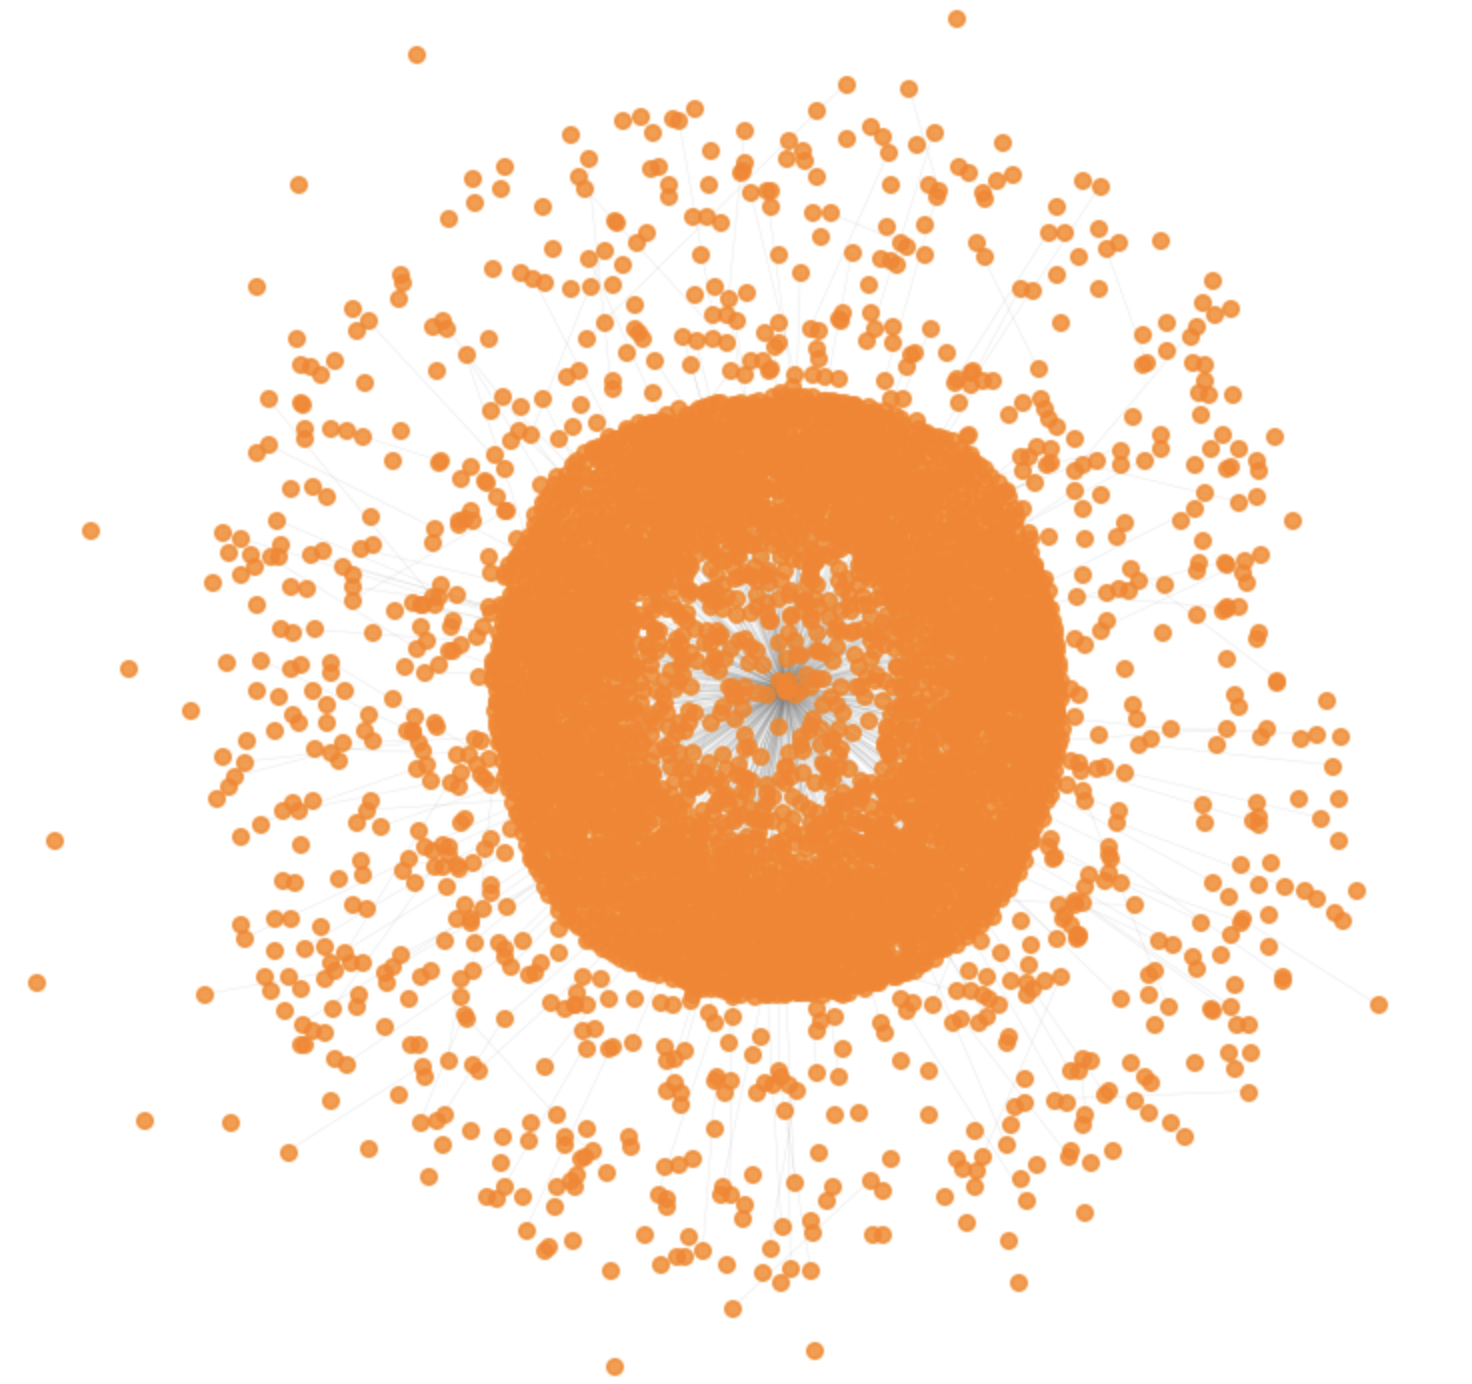
\includegraphics[width=\textwidth]{images/7.png}
	\end{center}
	\caption{Визуализация восьмого по величине сообщества (4 876 узлов)}
	\label{img:7}
\end{figure}

\clearpage
